% !TEX root=../main.tex

\renewcommand{\baselinestretch}{1.5}
\chapter{Baseline CNN Model}
\begin{figure}[htbp]
     \begin{subfigure}[b]{0.5\linewidth}
         \centering
		  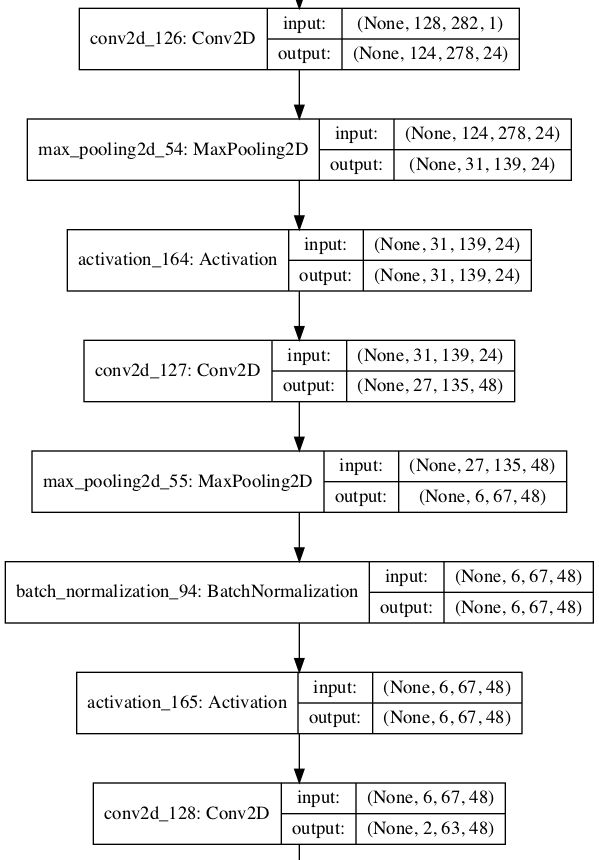
\includegraphics[scale=0.35]{Figs/Appen/simple_model_plot.png}
     \end{subfigure}
     ~
     \begin{subfigure}[b]{0.5\linewidth}
         \centering
		  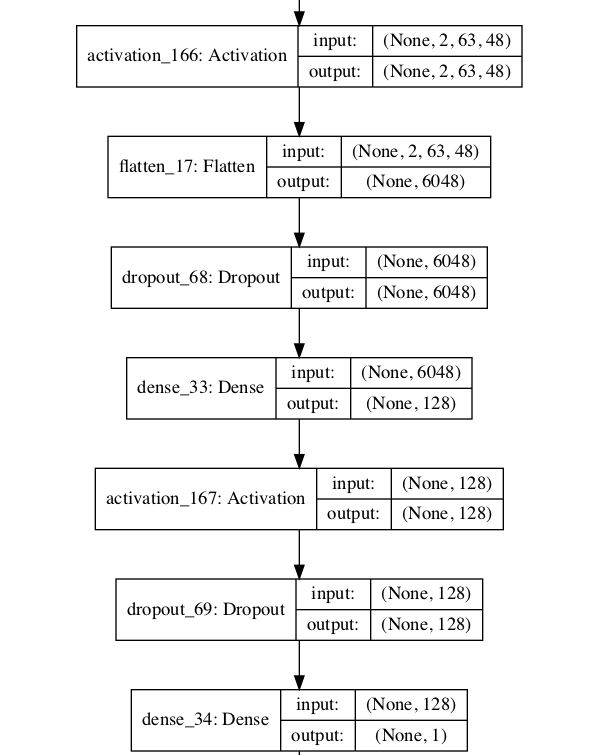
\includegraphics[scale=0.35]{Figs/Appen/simple_model_plot2.png}
     \end{subfigure}
  \caption{Structure of baseline model}
  \label{Fig:shapebaseline}
\end{figure}
\chapter{VGG-based CNN Model}
\begin{figure}[htbp]
      \centering
      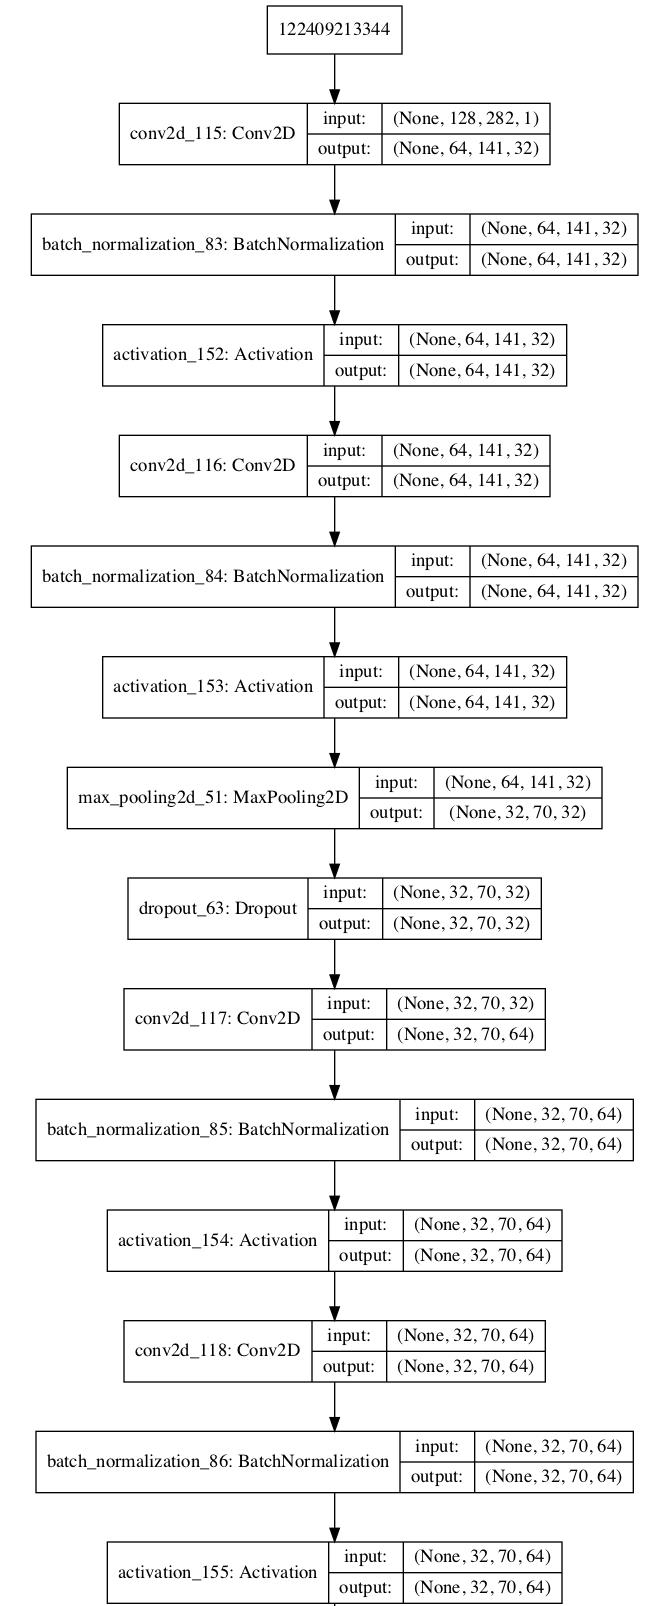
\includegraphics[scale=0.35]{Figs/Appen/model_plot1.png}
\end{figure}
\begin{figure}[htbp]
\centering
     \begin{subfigure}[b]{0.45\linewidth}
      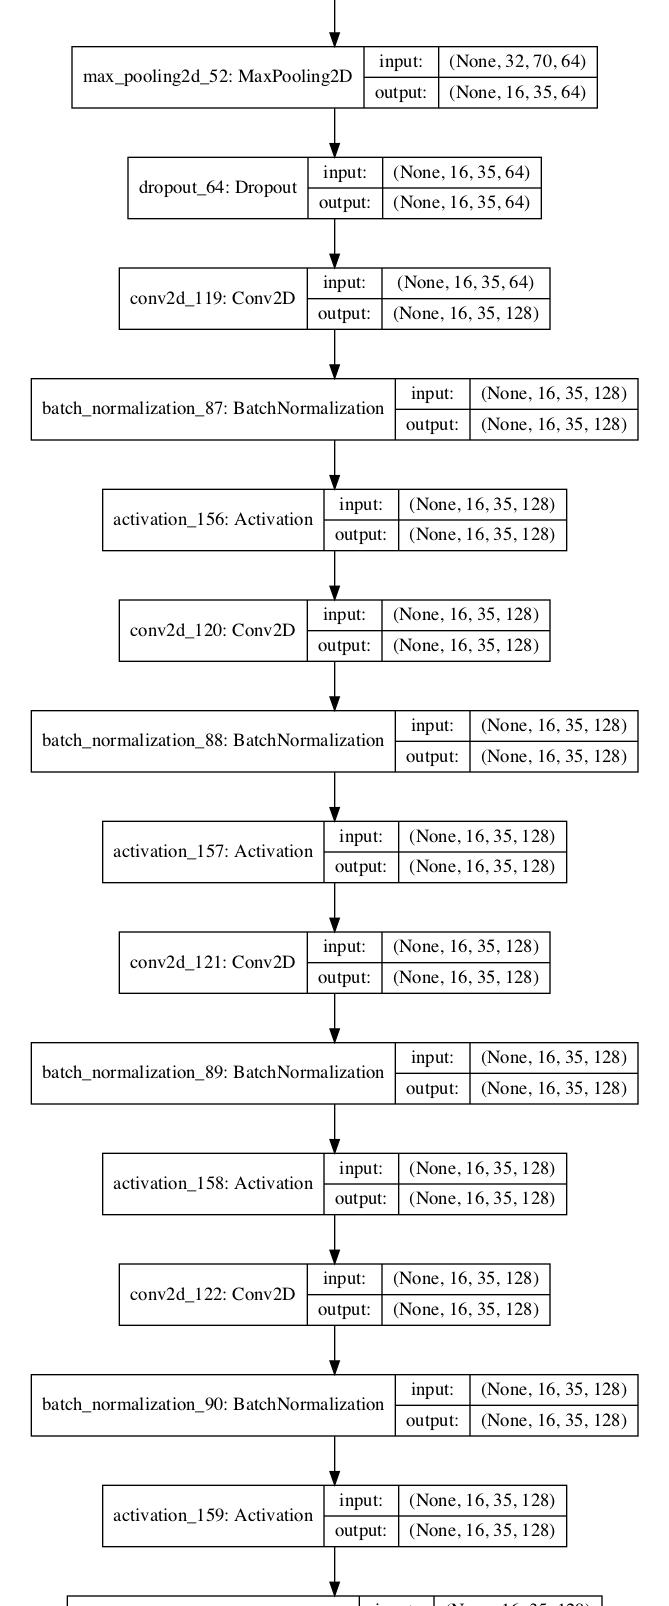
\includegraphics[scale=0.35]{Figs/Appen/model_plot2.png}
     \end{subfigure}
          \begin{subfigure}[b]{0.45\linewidth}
      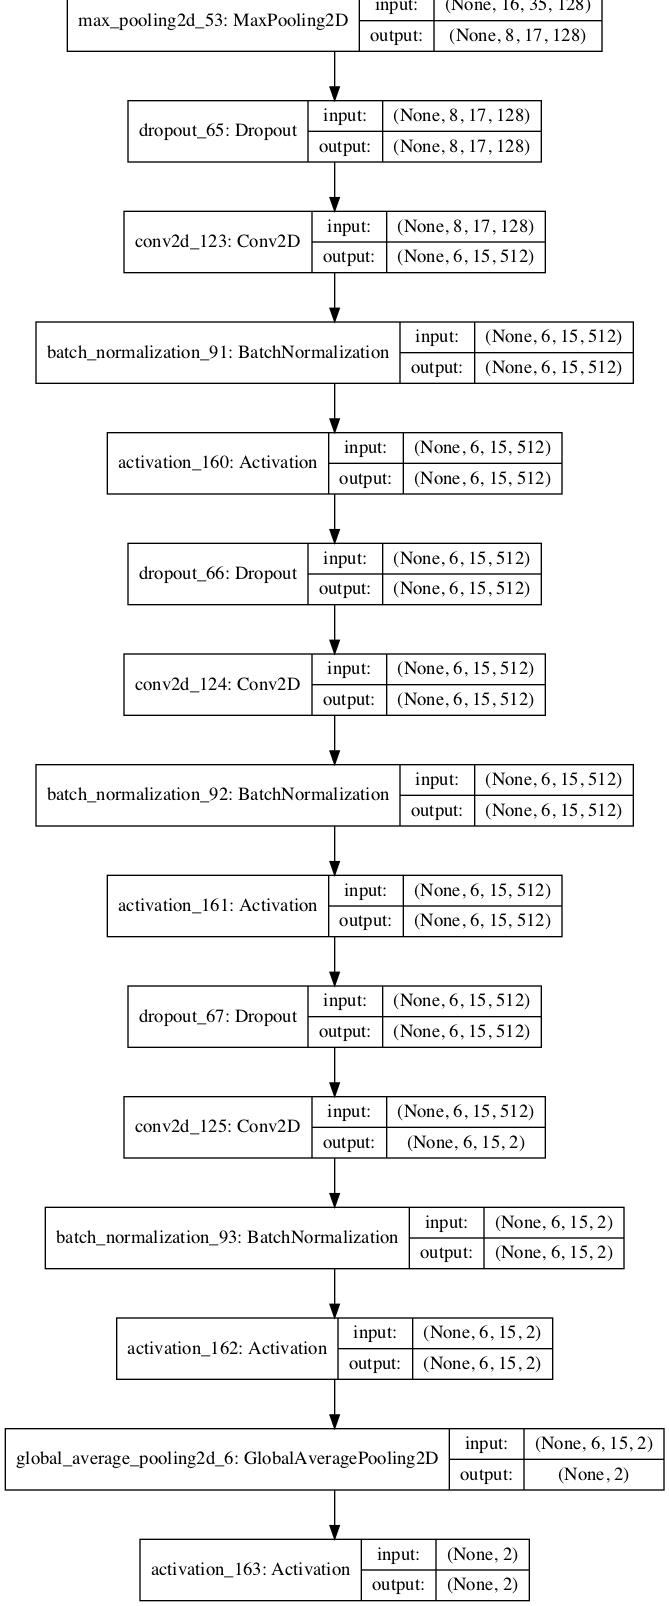
\includegraphics[scale=0.35]{Figs/Appen/model_plot3.png}
     \end{subfigure}
  \caption{Structure of VGG-based model}
  \label{Fig:shapevgg}
\end{figure}